\section{Results}

\subsection{Scaffold separation alone does not guarantee a clean benchmark split}

The first question was whether scaffold-based splitting changes only chemical overlap, or whether it also changes other properties of the benchmark. Table~\ref{tab:split-diagnostics} shows that ordinary scaffold splitting successfully removes scaffold overlap: across all datasets, the number of shared train/test scaffolds is zero. In contrast, random splitting produces substantial scaffold sharing. For example, random splitting shares approximately 100 test scaffolds in BACE, 111 in BBBP, and more than 2,300 in HIV.

However, removing scaffold overlap does not make the split automatically easy to interpret. Ordinary scaffold splitting can create strong target distribution shifts and highly concentrated test sets. This is especially visible in ESOL and FreeSolv. ESOL has only one test scaffold under the ordinary scaffold split and a target mean gap of 1.5734. FreeSolv is even more constrained: the largest scaffold accounts for nearly half of the dataset, the ordinary scaffold split has only one test scaffold, and the target mean gap reaches 2.8410. These cases show why a scaffold split should be described not only as ``non-overlapping'', but also in terms of target shift and scaffold concentration.

Target-balanced scaffold splitting reduces this problem in several datasets. In BACE, BBBP, ClinTox, and HIV, the target mean gap under balanced scaffold splitting is close to zero. ESOL also improves substantially relative to the ordinary scaffold split. FreeSolv remains problematic, with a balanced target gap of -1.2260, because the dataset is small and dominated by a large scaffold group. This exception is important: target balancing is useful as a diagnostic counterfactual, but it cannot always overcome structural constraints in the data.

\begin{table}[H]
\centering
\caption{Split diagnostics and scaffold statistics. Shared scaffold fraction is calculated relative to the test scaffold set.}
\label{tab:split-diagnostics}
\resizebox{\textwidth}{!}{%
\begin{tabular}{lllrrrrrr}
\toprule
Dataset & Task & Split & Scaffolds & Largest frac. & Singleton frac. & Test scaffolds & Shared scaffolds & Target gap \\
\midrule
BACE & Classification & Ordinary scaffold & 671.0 & 0.0364 & 0.7094 & 10.0 & 0.0 & 0.1854 \\
BACE & Classification & Random & 670.0 & 0.0364 & 0.7104 & 199.6 & 100.0 & -0.0016 \\
BACE & Classification & Balanced scaffold & 671.0 & 0.0364 & 0.7094 & 22.6 & 0.0 & -0.0014 \\
BBBP & Classification & Ordinary scaffold & 1025.0 & 0.0658 & 0.7620 & 8.0 & 0.0 & 0.1274 \\
BBBP & Classification & Random & 1024.0 & 0.0658 & 0.7627 & 271.6 & 111.0 & -0.0006 \\
BBBP & Classification & Balanced scaffold & 1025.0 & 0.0658 & 0.7620 & 22.4 & 0.0 & 0.0016 \\
ClinTox & Classification & Ordinary scaffold & 784.0 & 0.0992 & 0.7793 & 3.0 & 0.0 & -0.0595 \\
ClinTox & Classification & Random & 783.0 & 0.0992 & 0.7803 & 204.2 & 82.2 & 0.0015 \\
ClinTox & Classification & Balanced scaffold & 784.0 & 0.0992 & 0.7793 & 24.8 & 0.0 & -0.0006 \\
ESOL & Regression & Ordinary scaffold & 269.0 & 0.2829 & 0.7323 & 1.0 & 0.0 & 1.5734 \\
ESOL & Regression & Random & 268.0 & 0.2265 & 0.7351 & 78.6 & 36.0 & 0.0686 \\
ESOL & Regression & Balanced scaffold & 269.0 & 0.2829 & 0.7323 & 31.6 & 0.0 & 0.1062 \\
FreeSolv & Regression & Ordinary scaffold & 63.0 & 0.4984 & 0.5714 & 1.0 & 0.0 & 2.8410 \\
FreeSolv & Regression & Random & 62.0 & 0.2368 & 0.5806 & 23.2 & 15.0 & 0.2318 \\
FreeSolv & Regression & Balanced scaffold & 63.0 & 0.4984 & 0.5714 & 1.0 & 0.0 & -1.2260 \\
HIV & Classification & Ordinary scaffold & 19082.0 & 0.0508 & 0.7493 & 81.0 & 0.0 & -0.0039 \\
HIV & Classification & Random & 19081.0 & 0.0508 & 0.7494 & 5286.4 & 2363.6 & 0.0001 \\
HIV & Classification & Balanced scaffold & 19082.0 & 0.0508 & 0.7493 & 307.8 & 0.0 & -0.0037 \\
\bottomrule
\end{tabular}%
}
\end{table}

\subsection{Performance gaps shrink in some datasets after target balancing, but not universally}

The second question was whether performance gaps under ordinary scaffold splitting are partly explained by target shift. Figure~\ref{fig:gap} and Table~\ref{tab:gap} show that the answer is dataset- and model-dependent. In BBBP and ClinTox, Logistic Regression and Random Forest show smaller gaps after target balancing. In ESOL, tree-based models show a particularly large reduction: the Random Forest gap decreases from 1.038 to 0.340 RMSE, and the XGBoost gap decreases from 0.974 to 0.207 RMSE. This suggests that a substantial part of the ordinary scaffold gap in ESOL is associated with target shift rather than scaffold separation alone.

At the same time, the results caution against treating target-balanced scaffold splitting as simply ``better''. In HIV, balanced scaffold gaps are larger than ordinary scaffold gaps for all three classification models. In FreeSolv, Random Forest shows a negative balanced gap, while Ridge and XGBoost behave differently. These patterns show that target balancing changes the diagnostic question rather than providing a universal ranking of split difficulty. The important result is therefore not that one split is always preferable, but that the interpretation of model performance changes when target shift is measured and controlled.

\begin{figure}[H]
\centering
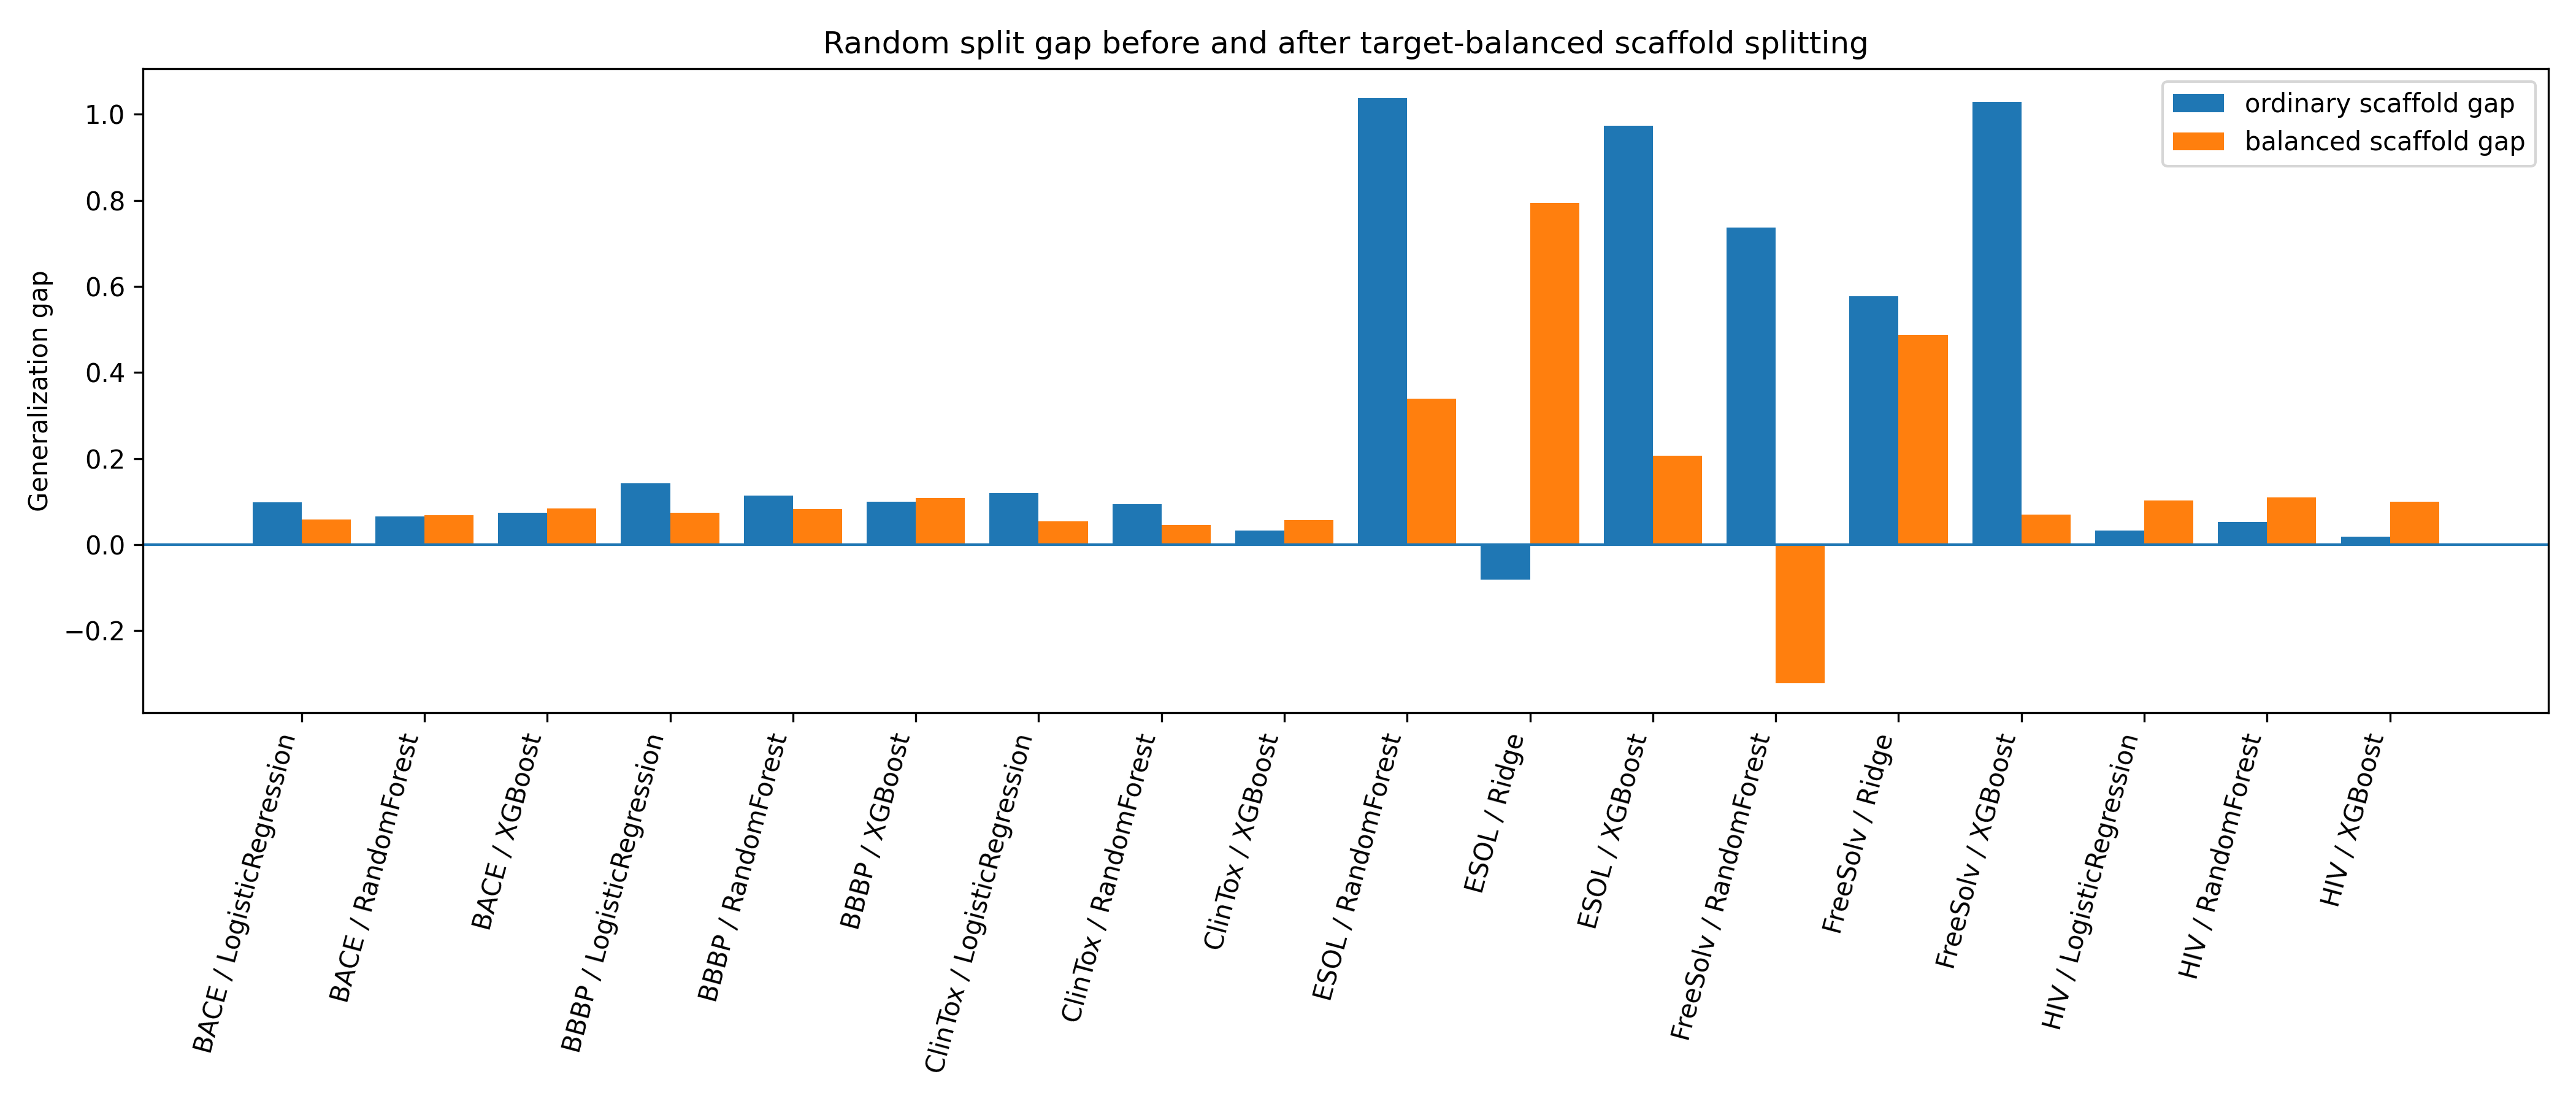
\includegraphics[width=\textwidth]{../paper1_leakage_benchmark/figures/figure1_gap_ordinary_vs_balanced.png}
\caption{Generalization gap under ordinary scaffold and target-balanced scaffold splitting. Classification gaps are random ROC-AUC minus scaffold ROC-AUC. Regression gaps are scaffold RMSE minus random RMSE.}
\label{fig:gap}
\end{figure}

\begin{table}[H]
\centering
\caption{Generalization gap summary. Positive classification gaps indicate lower ROC-AUC under scaffold-based splitting. Positive regression gaps indicate higher RMSE under scaffold-based splitting.}
\label{tab:gap}
\resizebox{\textwidth}{!}{%
\begin{tabular}{llllrrr}
\toprule
Dataset & Task & Model & Metric & Ordinary gap & Balanced gap & Gap reduction \\
\midrule
BACE & Classification & LogisticRegression & ROC-AUC & 0.098 & 0.058 & 0.040 \\
BACE & Classification & RandomForest & ROC-AUC & 0.065 & 0.069 & -0.004 \\
BACE & Classification & XGBoost & ROC-AUC & 0.074 & 0.084 & -0.010 \\
BBBP & Classification & LogisticRegression & ROC-AUC & 0.143 & 0.074 & 0.068 \\
BBBP & Classification & RandomForest & ROC-AUC & 0.114 & 0.082 & 0.031 \\
BBBP & Classification & XGBoost & ROC-AUC & 0.100 & 0.109 & -0.009 \\
ClinTox & Classification & LogisticRegression & ROC-AUC & 0.119 & 0.054 & 0.065 \\
ClinTox & Classification & RandomForest & ROC-AUC & 0.094 & 0.046 & 0.048 \\
ClinTox & Classification & XGBoost & ROC-AUC & 0.033 & 0.057 & -0.024 \\
ESOL & Regression & RandomForest & RMSE & 1.038 & 0.340 & 0.698 \\
ESOL & Regression & Ridge & RMSE & -0.082 & 0.793 & -0.875 \\
ESOL & Regression & XGBoost & RMSE & 0.974 & 0.207 & 0.767 \\
FreeSolv & Regression & RandomForest & RMSE & 0.737 & -0.323 & 1.060 \\
FreeSolv & Regression & Ridge & RMSE & 0.577 & 0.487 & 0.091 \\
FreeSolv & Regression & XGBoost & RMSE & 1.029 & 0.069 & 0.959 \\
HIV & Classification & LogisticRegression & ROC-AUC & 0.033 & 0.103 & -0.070 \\
HIV & Classification & RandomForest & ROC-AUC & 0.053 & 0.110 & -0.057 \\
HIV & Classification & XGBoost & ROC-AUC & 0.018 & 0.100 & -0.082 \\
\bottomrule
\end{tabular}%
}
\end{table}

\subsection{Random splits are chemically closer to the training set}

The third question was whether random splits produce chemically easier test sets. Figure~\ref{fig:tanimoto} and Table~\ref{tab:similarity} show a consistent pattern: random split test molecules have higher maximum Tanimoto similarity to training molecules than scaffold-based test molecules. This holds across both classification and regression datasets. For example, mean maximum Tanimoto similarity under random splitting is 0.791 for BACE, 0.564 for BBBP, 0.556 for ESOL, 0.544 for FreeSolv, and 0.616 for HIV.

Ordinary scaffold splitting usually produces the lowest similarity, especially in ESOL and FreeSolv. Balanced scaffold splitting often lies between random and ordinary scaffold splitting. This intermediate behavior is useful diagnostically: it helps distinguish the effect of target balancing from the effect of maximizing chemical dissimilarity. Together with the performance-gap results, the similarity audit shows why aggregate scores alone are insufficient. A model score is more interpretable when accompanied by information about how chemically close the test molecules are to the training set.

\begin{figure}[H]
\centering
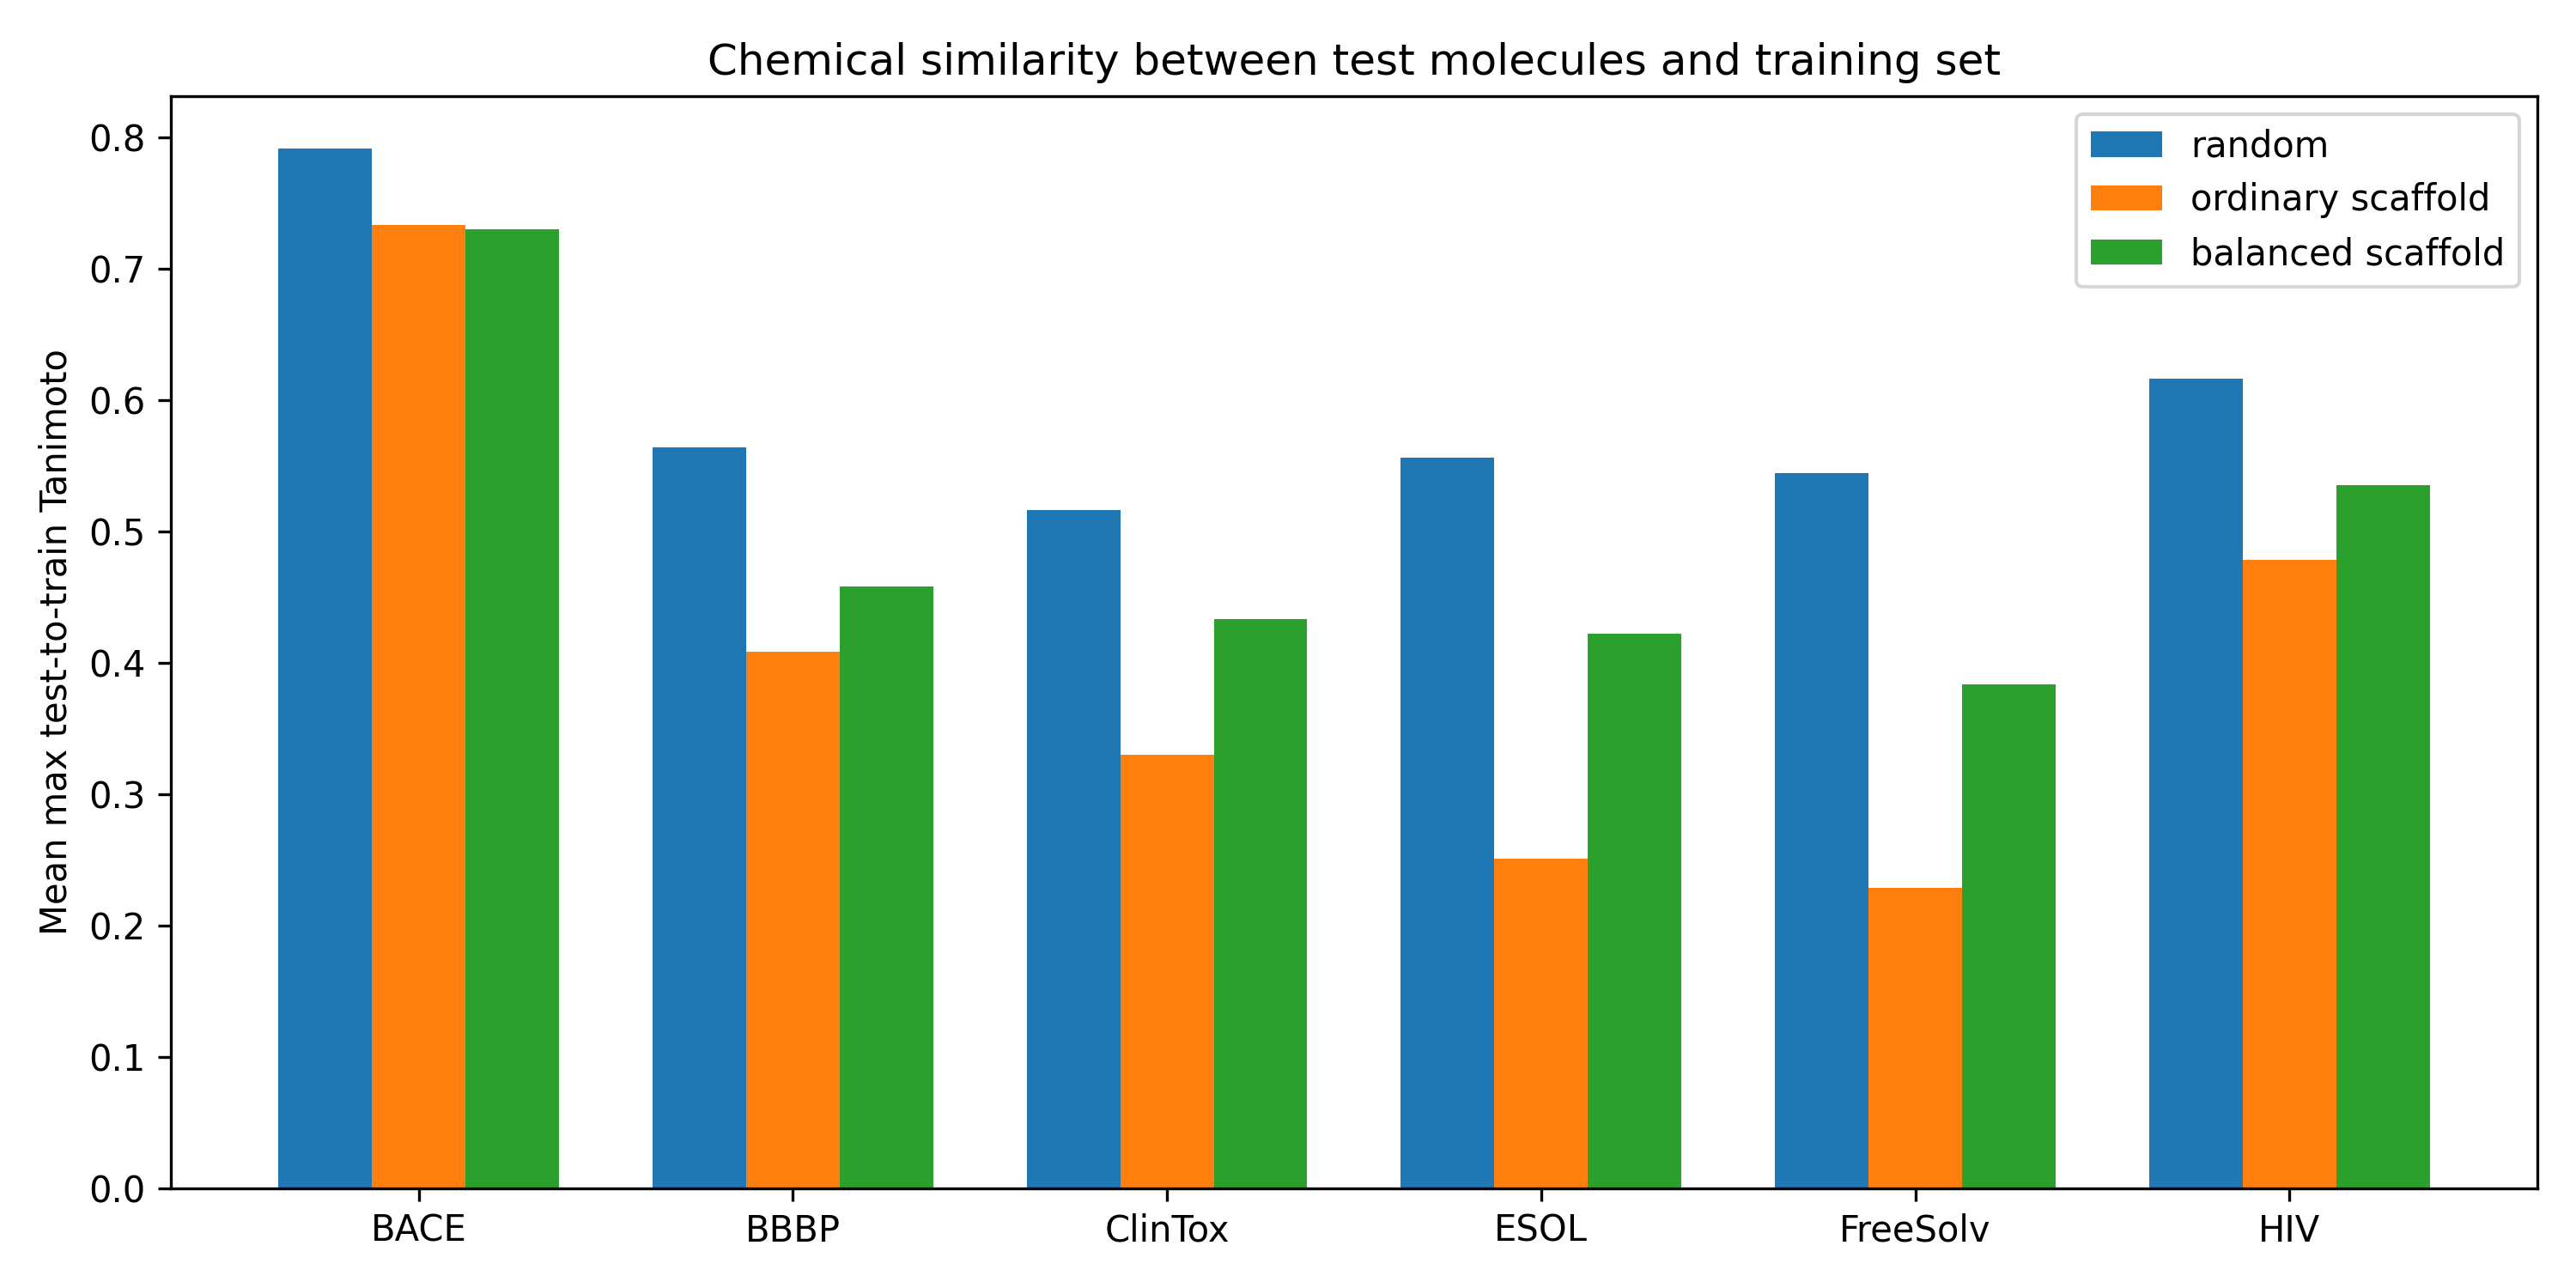
\includegraphics[width=0.95\textwidth]{../paper1_leakage_benchmark/figures/figure3_tanimoto_similarity.png}
\caption{Mean maximum test-to-train Tanimoto similarity by split strategy. Random splits generally create more chemically similar train/test pairs than scaffold-based splits.}
\label{fig:tanimoto}
\end{figure}

\begin{table}[H]
\centering
\caption{Test-to-train Tanimoto similarity audit. Values are based on maximum similarity from each test molecule to the training set.}
\label{tab:similarity}
\resizebox{\textwidth}{!}{%
\begin{tabular}{lllrrrr}
\toprule
Dataset & Task & Split & Mean max & Median max & P90 max & Fraction $\geq 0.8$ \\
\midrule
BACE & Classification & Balanced scaffold & 0.730 & 0.735 & 0.824 & 0.181 \\
BACE & Classification & Ordinary scaffold & 0.733 & 0.740 & 0.834 & 0.199 \\
BACE & Classification & Random & 0.791 & 0.807 & 0.911 & 0.538 \\
BBBP & Classification & Balanced scaffold & 0.458 & 0.436 & 0.677 & 0.009 \\
BBBP & Classification & Ordinary scaffold & 0.409 & 0.403 & 0.660 & 0.000 \\
BBBP & Classification & Random & 0.564 & 0.570 & 0.793 & 0.096 \\
ClinTox & Classification & Balanced scaffold & 0.433 & 0.409 & 0.640 & 0.008 \\
ClinTox & Classification & Ordinary scaffold & 0.330 & 0.305 & 0.556 & 0.007 \\
ClinTox & Classification & Random & 0.516 & 0.493 & 0.797 & 0.098 \\
ESOL & Regression & Balanced scaffold & 0.422 & 0.388 & 0.630 & 0.033 \\
ESOL & Regression & Ordinary scaffold & 0.251 & 0.240 & 0.359 & 0.000 \\
ESOL & Regression & Random & 0.556 & 0.548 & 0.817 & 0.110 \\
FreeSolv & Regression & Balanced scaffold & 0.384 & 0.370 & 0.500 & 0.000 \\
FreeSolv & Regression & Ordinary scaffold & 0.228 & 0.222 & 0.320 & 0.000 \\
FreeSolv & Regression & Random & 0.544 & 0.522 & 0.827 & 0.113 \\
HIV & Classification & Balanced scaffold & 0.535 & 0.519 & 0.722 & 0.040 \\
HIV & Classification & Ordinary scaffold & 0.478 & 0.466 & 0.680 & 0.022 \\
HIV & Classification & Random & 0.616 & 0.630 & 0.833 & 0.155 \\
\bottomrule
\end{tabular}%
}
\end{table}

\subsection{Split diagnostics change how model comparisons should be read}

The final question was whether split choice changes only the magnitude of performance or also the interpretation of model comparison. The appendix ranking analysis shows that model rankings can change across random, ordinary scaffold, and balanced scaffold protocols. This matters because benchmark papers often use rankings to support claims about method superiority. If the best-performing model changes when the split changes, then a leaderboard-style conclusion is incomplete without split diagnostics.

Overall, the results support the central story of this paper. Random splitting often produces chemically closer test sets. Ordinary scaffold splitting removes scaffold overlap but can introduce target shift and scaffold concentration. Target-balanced scaffold splitting helps separate target-shift effects from scaffold-generalization effects, but does not eliminate all dataset- and model-dependent behavior. Therefore, molecular property prediction benchmarks should report the properties of the split alongside model scores.
